\chapter{Ensayos y resultados}

\label{Chapter4}

En este capítulo se detallan los ensayos realizados al sistema completo y los resultados obtenidos durante las pruebas de funcionamiento.

\section{Banco de pruebas}

El sistema consta físicamente de dos tipos de componentes: nodos y servidor. El servidor incluye tanto la aplicación en el frontend y el backend con sus respectivos módulos. Además, el sistema posee dos tipos de nodos: uno para el control de calefacción y otro para el control de iluminación.

Para ensayar el nodo de temperatura, se utilizaron los materiales que lo conforman que se muestran en la figura \ref{fig:31}.

\begin{figure}[h]
\centering
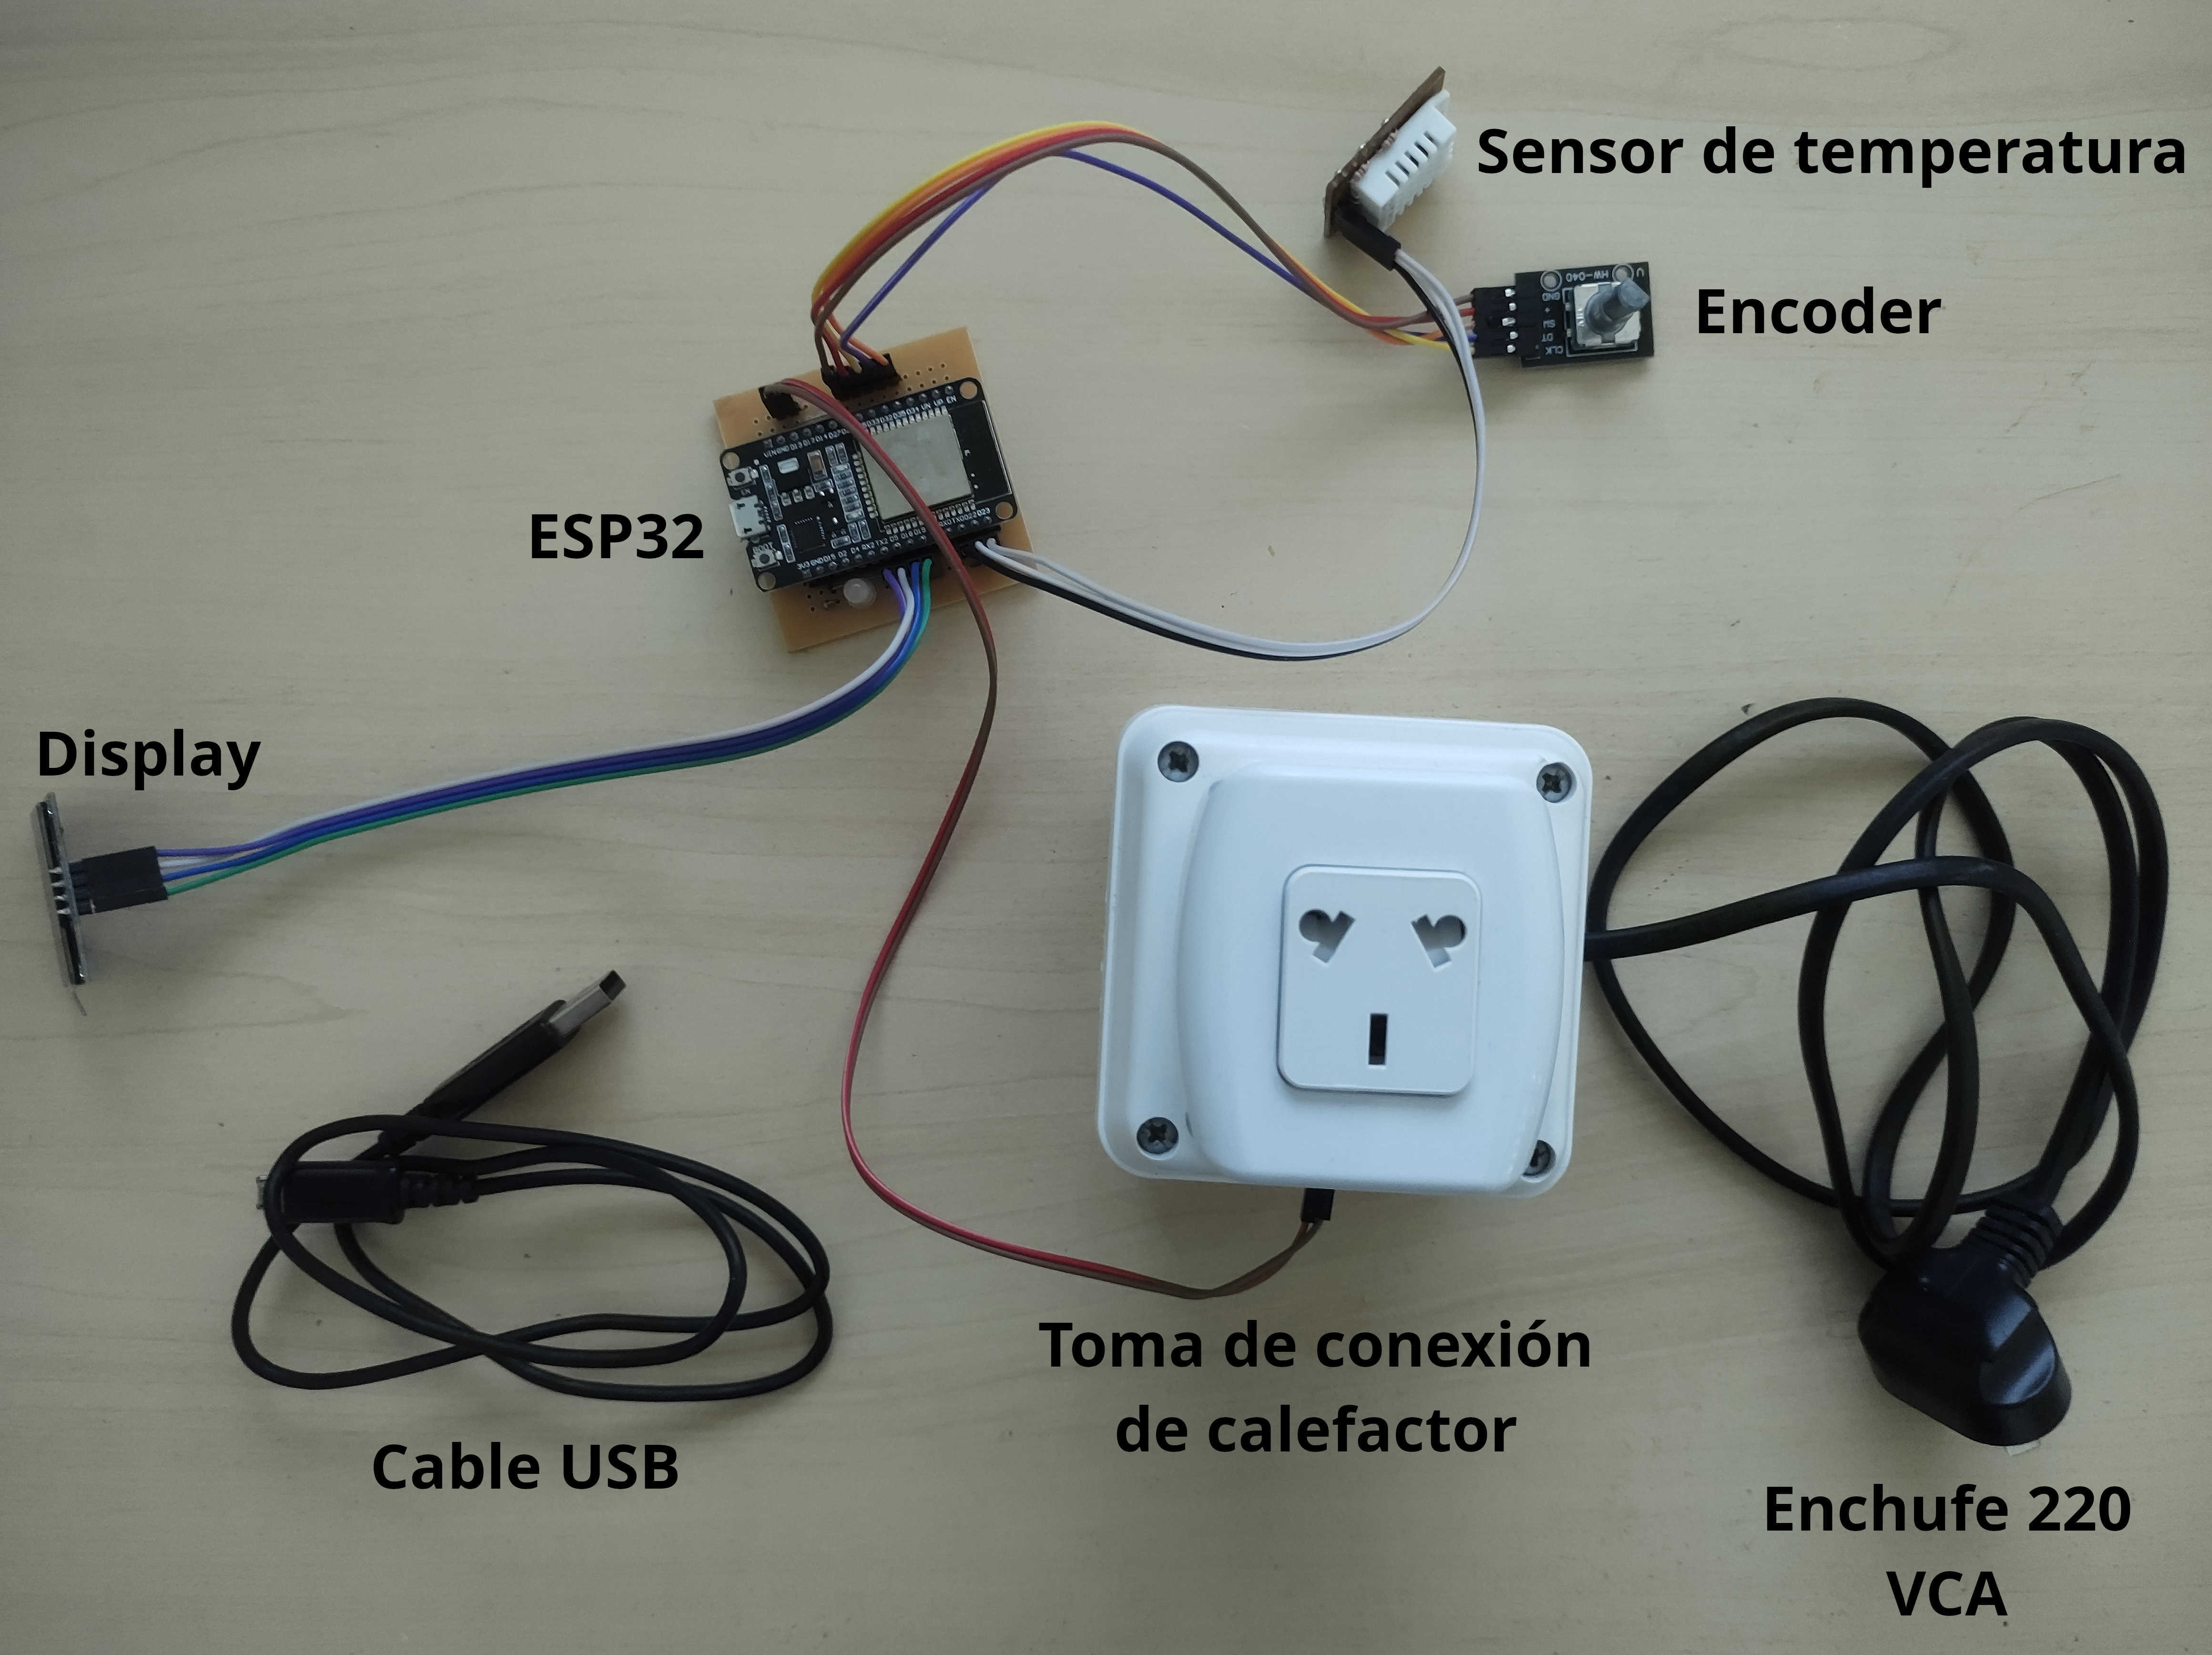
\includegraphics[scale=0.25]{Figura 31 - Nodo temperatura.jpg}
\caption[Componentes del nodo de temperatura]{Componentes del nodo de temperatura.}
\label{fig:31}
\end{figure}

En la figura \ref{fig:31}, se puede observar la placa ESP32 montada sobre la placa de conexiones, el display, el encoder, el sensor de temperatura y una caja estanca con una conexión de toma corriente para conectar la estufa a encender. Además, esta caja incluye un cable para conectarse a una fuente de alimentación de 220 VCA, que actúa como un interruptor. Cabe aclarar que en modo automático, el control de temperatura opera con una histéresis de 1 grado. Esto significa que al configurar una temperatura específica, el control apagará la salida cuando la temperatura supere en 1 grado al set-point y la encenderá cuando esté 1 grado por debajo de este valor.

Para ensayar el nodo de dimerización, se utilizaron los materiales que lo conforman que se muestran en la figura \ref{fig:32}.

\begin{figure}[h]
\centering
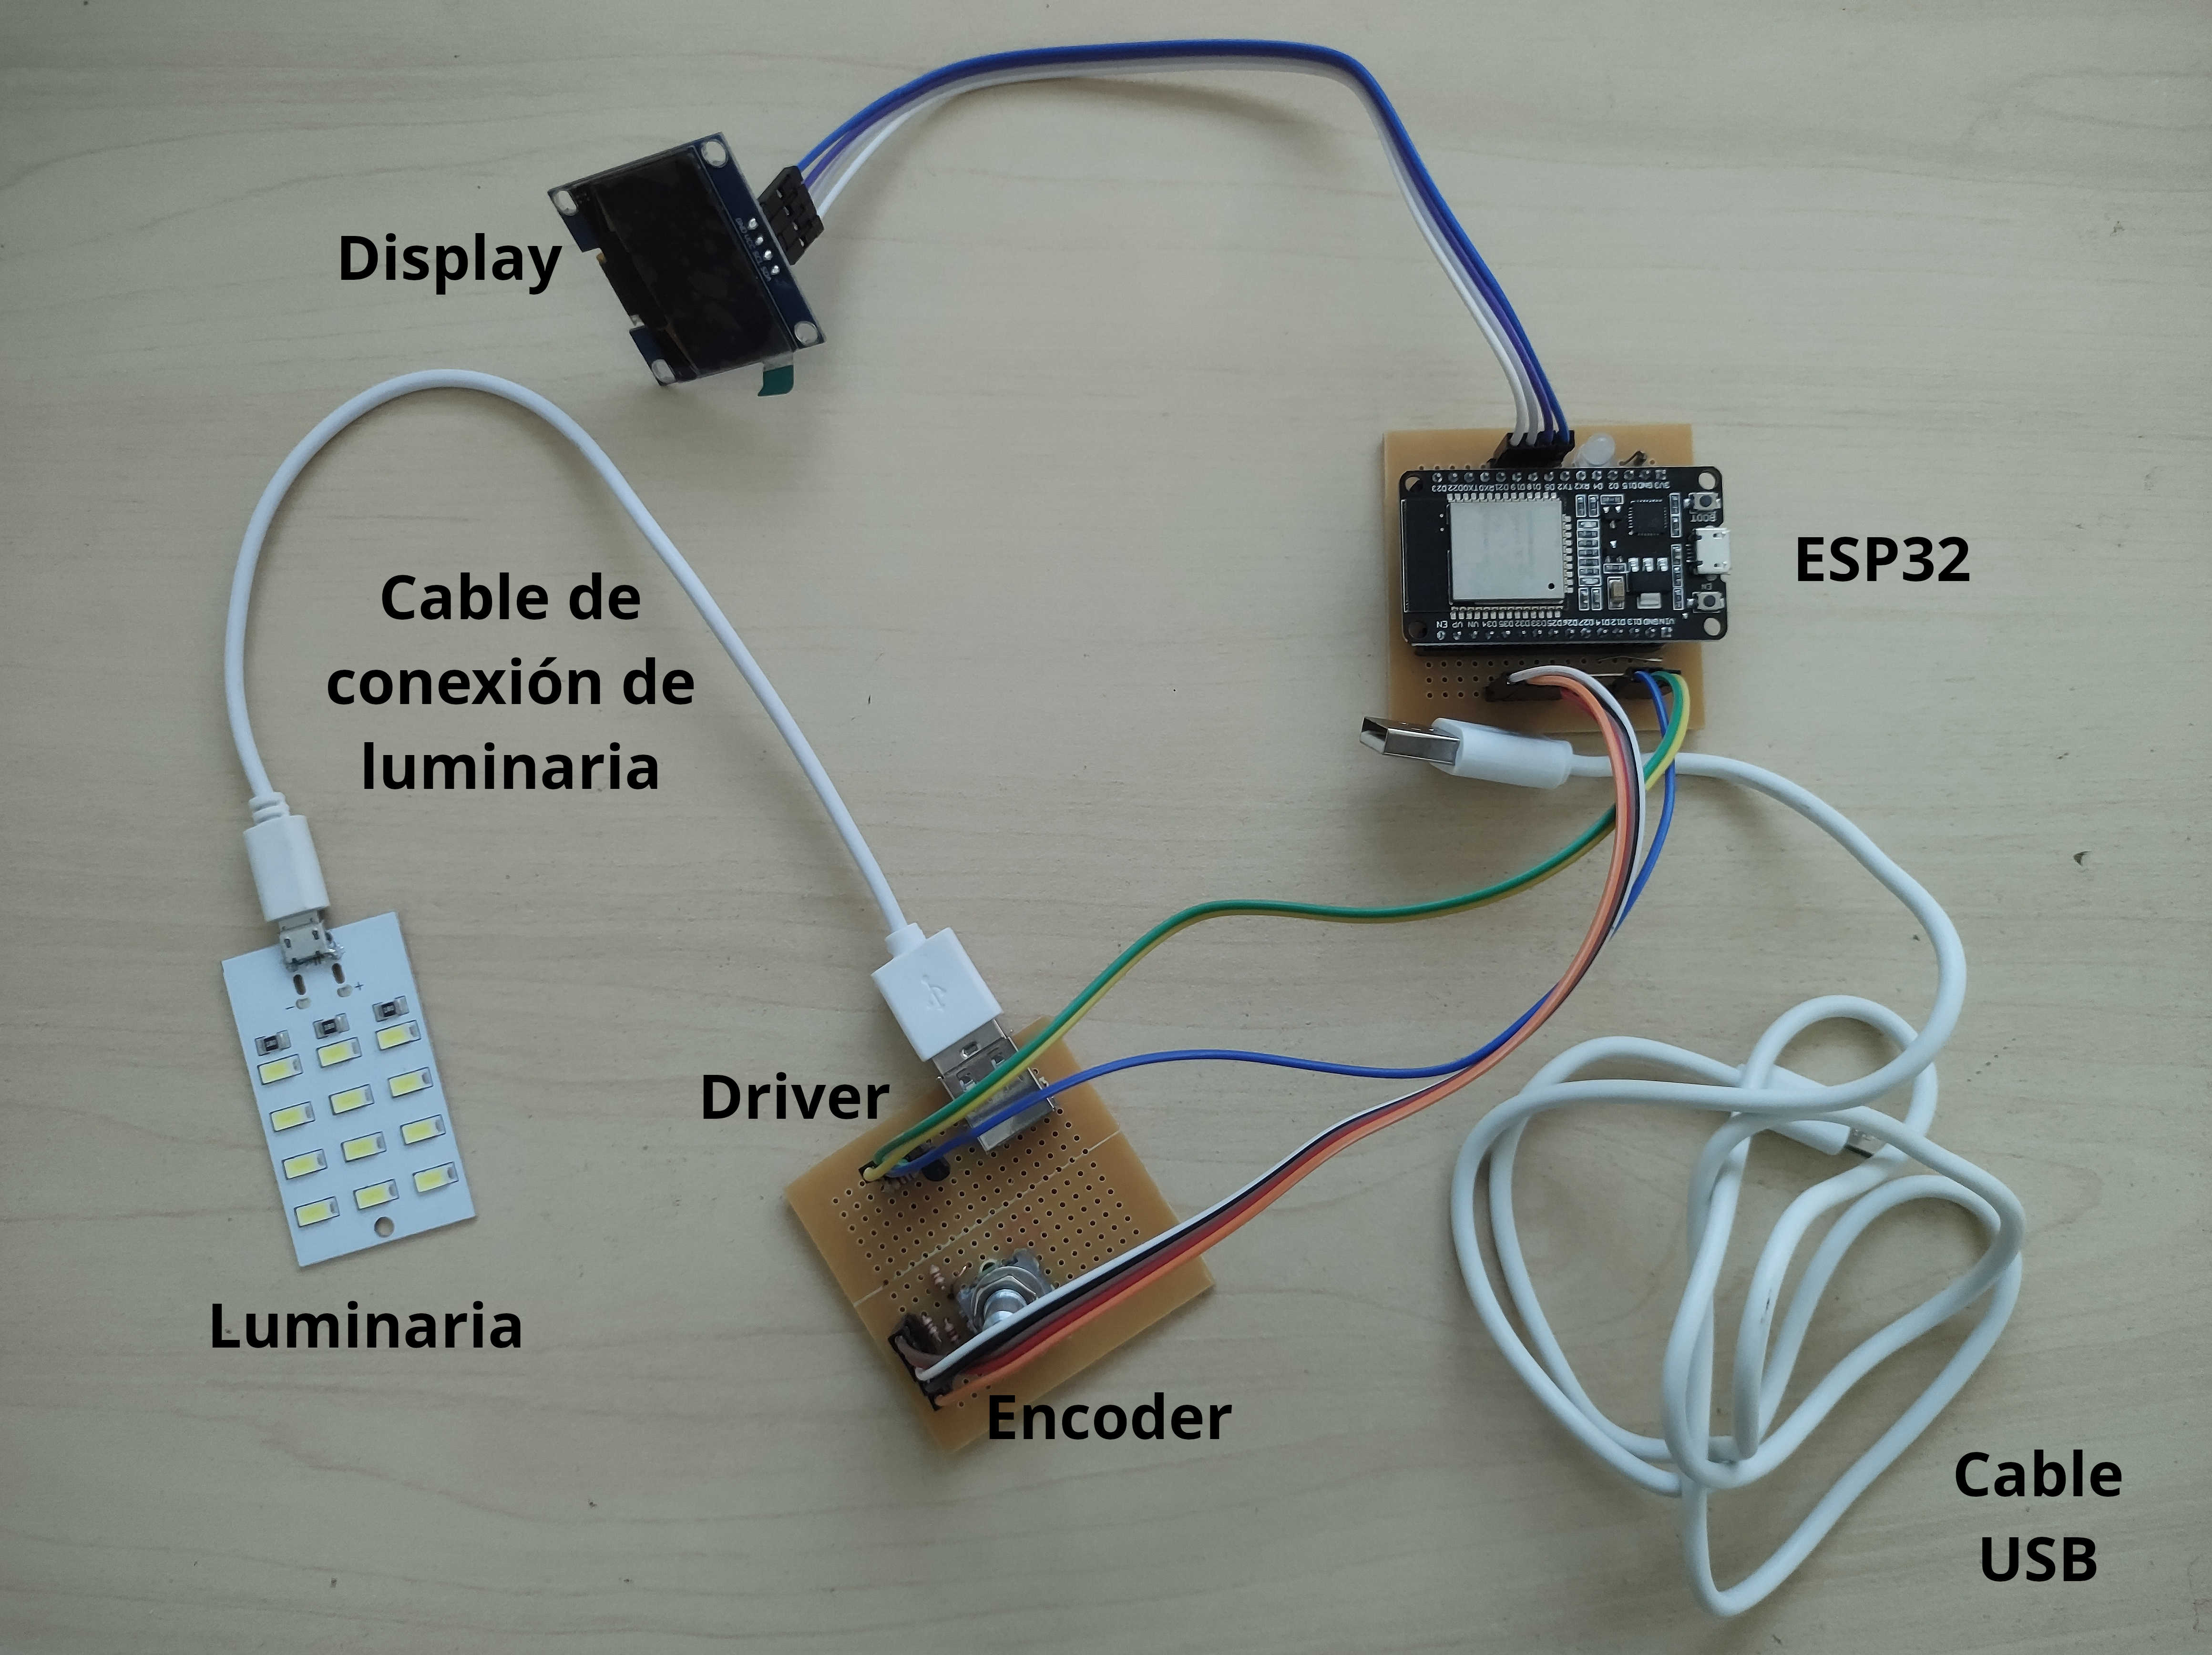
\includegraphics[scale=0.25]{Figura 32 - Nodo dimmer.jpg}
\caption[Componentes del nodo de dimerización]{Componentes del nodo de dimerización.}
\label{fig:32}
\end{figure}

En la figura  \ref{fig:32} se puede observar la placa ESP32 montada sobre la placa de conexiones, el display, el encoder, el \textit{driver} de iluminación y la placa de LEDs de 5 VCC. El control posee un conector USB por lo que puede conectarse cualquier lámpara que funcione en este caso con 5 VCC y posea este conector.

En la figura \ref{fig:33} pueden verse los componentes que forman parte del servidor.

\begin{figure}[h]
\centering
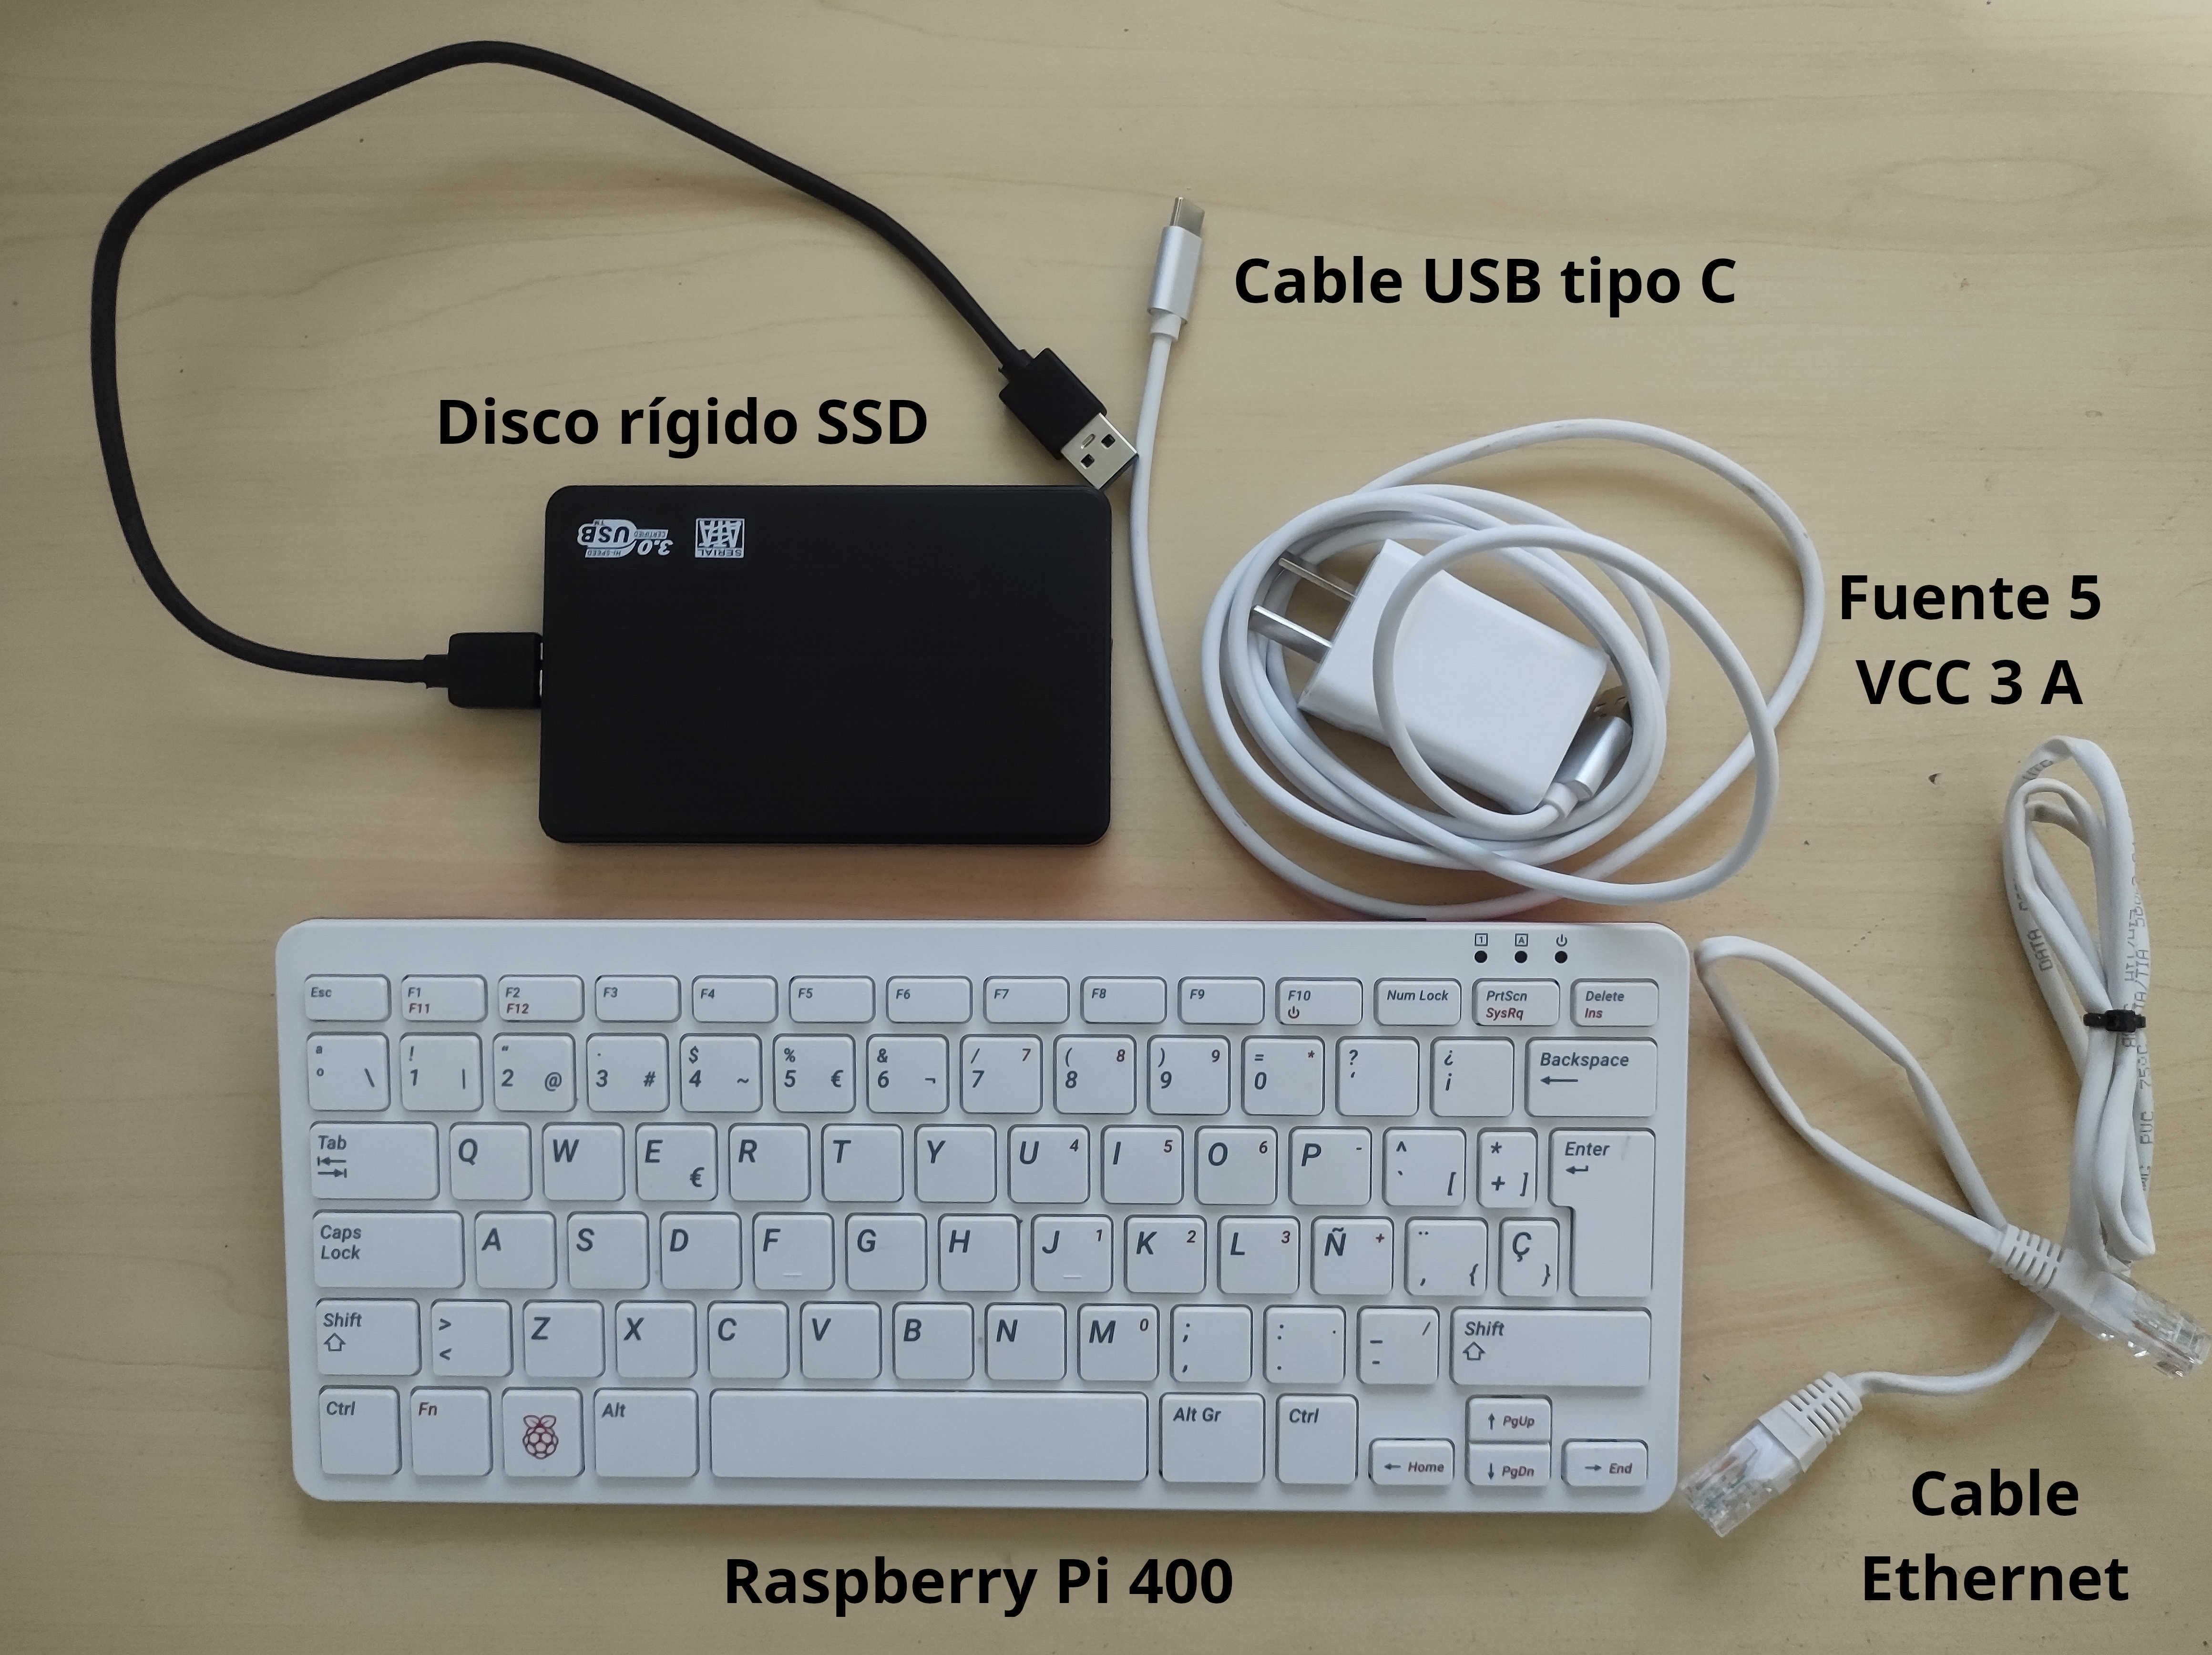
\includegraphics[scale=0.25]{Figura 33 - Servidor.jpg}
\caption[Componentes del servidor]{Componentes del servidor.}
\label{fig:33}
\end{figure}

Puede observarse la Raspberry Pi400, la fuente de 5 VCC 3A con su cable, un disco rígido externo SSD de 120 GB y un cable Ethernet para la conexión a la red.

\section{Metodología empleada}

El hardware se testeó de forma funcional. En cuanto al software se utilizaron distintas metodologías para la depuración de forma manual de los embebidos, el frontend y el backend. A continuación, se describen cada una de ellas.

\subsection{Pruebas del frontend}

Para el frontend se utilizaron pruebas funcionales manuales con el sistema funcionando. El desarrollo fue progresivo y se llevó a cabo en paralelo. Se creó una aplicación básica y, posteriormente, se fueron agregando nuevas funcionalidades. A medida que el sistema fue creciendo, se fueron agregando más componentes hasta tener la versión actual.

En lo que respecta a las pruebas, se empleó la salida de la consola del navegador a medida que se implementaban nuevas funciones y páginas. Esto permitió exhibir en tiempo real el funcionamiento del sistema en cada página y con cada función agregada. En el código \ref{lst:console front} se muestra a modo de ejemplo parte del desarrollo de la página para la visualización de un mensaje por consola de la configuración de un dispositivo.

\begin{lstlisting}[caption={Muestra por consola de los datos recibidos.}, label={lst:console front}]
ngOnInit() {
    const deviceId = this.activatedRoute.snapshot.paramMap.get('id') as string;
    this.dispositivoId = deviceId, 10;
    this.subscription = this.dispositivoService.getDeviceById(this.dispositivoId).
   		subscribe((data) => {
      console.log(data);
      this.device = data[0];
      this.tipo = data[0].tipo;
      this.ubicacion = data[0].ubicacion;
    });
    this.leerdatos();
  }
\end{lstlisting}

Allí se puede ver la función \textit{console.log} mostrando los datos por consola. En la figura \ref{fig:34} se puede ver la pantalla de configuración del dispositivo y el mensaje por consola con los datos recibidos.

\newpage
\begin{figure}[h]
\centering
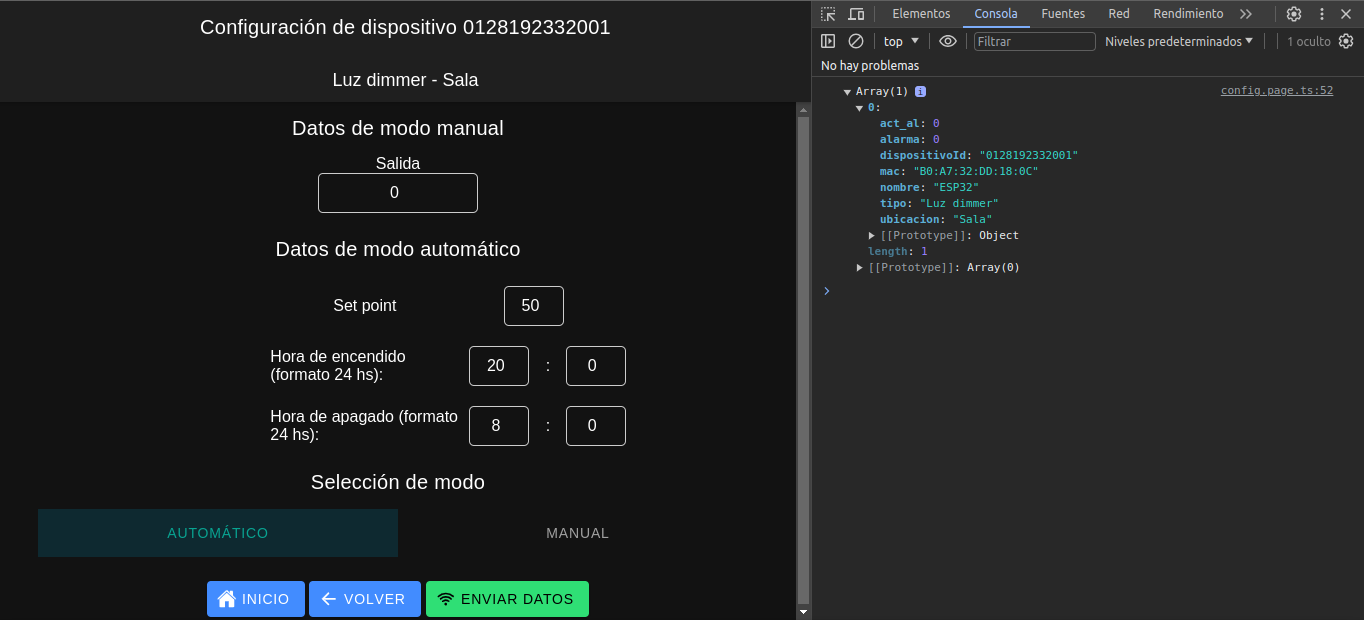
\includegraphics[scale=0.37]{Figura 34 - Consola front.png}
\caption[Pantalla de aplicación y consola del frontend]{Pantalla de aplicación y consola.}
\label{fig:34}
\end{figure}

Este mecanismo se utilizó en todas las páginas de la aplicación web y gracias a esto se consiguieron los resultados esperados de funcionalidad y depuración de errores.

\subsection{Pruebas del backend}

Para el backend se utilizó un mecanismo similar de pruebas funcionales que para el frontend.

El desarrollo siguió un enfoque progresivo lo que significa que a medida que se fueron incorporando funciones o endpoints nuevos, se fueron colocando muestras por consola para poder observar si los datos y las consultas estaban siendo resueltos de forma correcta. En el código \ref{lst:console back} se muestra como ejemplo el \textit{router} para borrar la tabla de mediciones de un dispositivo y el mensaje por consola de éxito y el ID del dispositivo.

\begin{lstlisting}[caption={Muestra por consola de los datos consultados.}, label={lst:console back}]
borrarTablaRouter.delete('/:id', async function (req, res, next) {
  const id = req.params.id;
  let connection;
  try {
      connection = await pool.getConnection();
      await connection.beginTransaction();
      const deleteMedicionesQuery = 'DELETE FROM Mediciones WHERE dispositivoId = ?';
      await connection.query(deleteMedicionesQuery, id);
      await connection.commit();
      connection.release();
      res.send({ message: 'Mediciones eliminadas exitosamente' }).status(200);
      console.log('Solicitud de eliminacion recibida para dispositivoId:', id);
      } catch (err) {
          if (connection) {
              await connection.rollback();
              connection.release();
          }
          res.send(err).status(400);
          console.log('Error al eliminar mediciones:', err);
      }
  });
\end{lstlisting}

En la figura \ref{fig:35} se puede ver la consola con el mensaje de éxito y el ID del dispositivo cuya tabla de mediciones fue eliminada.

\begin{figure}[h]
\centering
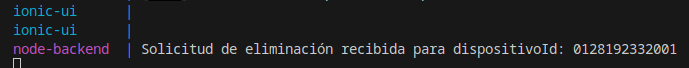
\includegraphics[scale=0.65]{Figura 35 - Consola back.png}
\caption[Mensaje por consola del servidor en el backend]{Mensaje por consola del servidor.}
\label{fig:35}
\end{figure}

Además de estas pruebas, se incorporó el uso de la aplicación \textit{MQTTX} para testear la comunicación con el \textit{broker} y los dispositivos, especialmente durante la implementación de la seguridad con los certificados SSL. De esta forma, se llevaron a cabo pruebas que abarcaron desde la primera conexión segura hasta la inserción de datos desde un dispositivo simulado, el envío de configuración desde la aplicación a los nodos y el mensaje de solicitud de configuración inicial de un nodo, entre otros.

En la figura \ref{fig:36} puede verse la configuración de \textit{MQTTX} para el envío de datos de una medición simulada en el \textit{topic \textbackslash home\textbackslash temperatura\textbackslash data} para luego verificar la correcta inserción en la base de datos.

\begin{figure}[h]
\centering
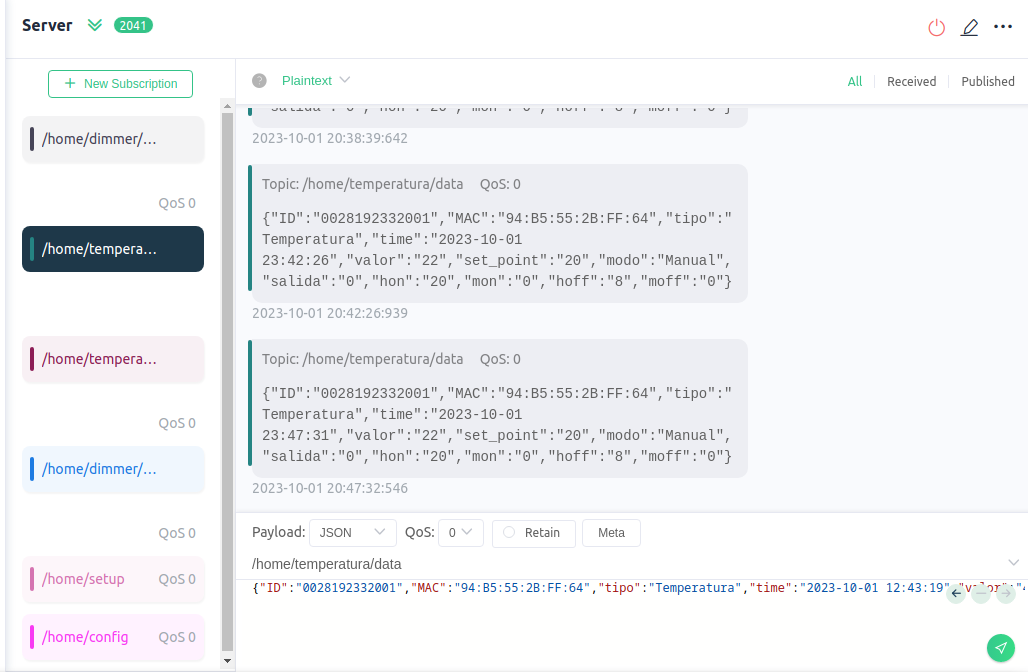
\includegraphics[scale=0.5]{Figura 36 - MQTTX.png}
\caption[Pantalla de MQTTX]{Pantalla de MQTTX.}
\label{fig:36}
\end{figure}

\subsection{Pruebas de los nodos}

El hardware se testeó haciendo pruebas de funcionamiento con los materiales mencionados en la sección anterior. Las pruebas consistieron en poner en funcionamiento los nodos durante dos días consecutivos, verificando que el control de temperatura funcionara dentro de los valores configurados y que la luminaria se encendiera y mantuviera los valores de los saltos. También se evaluó el funcionamiento de los horarios de encendido y apagado.

En cuanto al software, las placas ESP32 poseen comunicación serial incorporada por lo que se colocaron funciones de muestra por consola al momento de incorporar funcionalidades nuevas. En el código \ref{lst:dispositivo}, se puede ver un ejemplo de cómo se utilizó la función \textit{ESP\_LOGI} para mostrar por consola el valor de la salida recibido por MQTT.

\lstset{frame=tb,
  language=C++,
  aboveskip=3mm,
  belowskip=3mm,
  captionpos=b,
  showstringspaces=false,
  columns=flexible,
  basicstyle={\small\ttfamily},
  numbers=left,
  numberstyle=\tiny\color{gray},
  keywordstyle=\color{blue},
  commentstyle=\color{dkgreen},
  stringstyle=\color{mauve},
  breaklines=true,
  breakatwhitespace=true,
  tabsize=3,
}

\begin{lstlisting}[caption={Muestra por consola de la terminal ESP-IDF.}, label={lst:dispositivo}]
const cJSON *salida = cJSON_GetObjectItemCaseSensitive(root, "salida");
    if (cJSON_IsNumber(salida) && select) {
        if(salida->valueint==100)
            out_temp=true;
        if(salida->valueint==0)
            out_temp=false;
        ESP_LOGI(TAG, "Received MQTT salida: %d", salida->valueint);
        pant_main();
    }
\end{lstlisting}

En este caso se muestra por consola el mensaje de recepción del valor de salida y su valor correspondiente.

\section{Resultados finales}

Para la prueba final, se ensamblaron los 2 nodos, y se conectó un calefactor eléctrico de 750 W al nodo de temperatura. En el lado del servidor, se ejecutó el \textit{docker-compose} con el sistema completo. Se realizaron ajustes tanto desde la aplicación web como de cada uno de los nodos.

En la figura \ref{fig:37}, se puede observar el nodo de iluminación funcionando encendido, y en la pantalla se muestra el valor de la salida.

\begin{figure}[h]
\centering
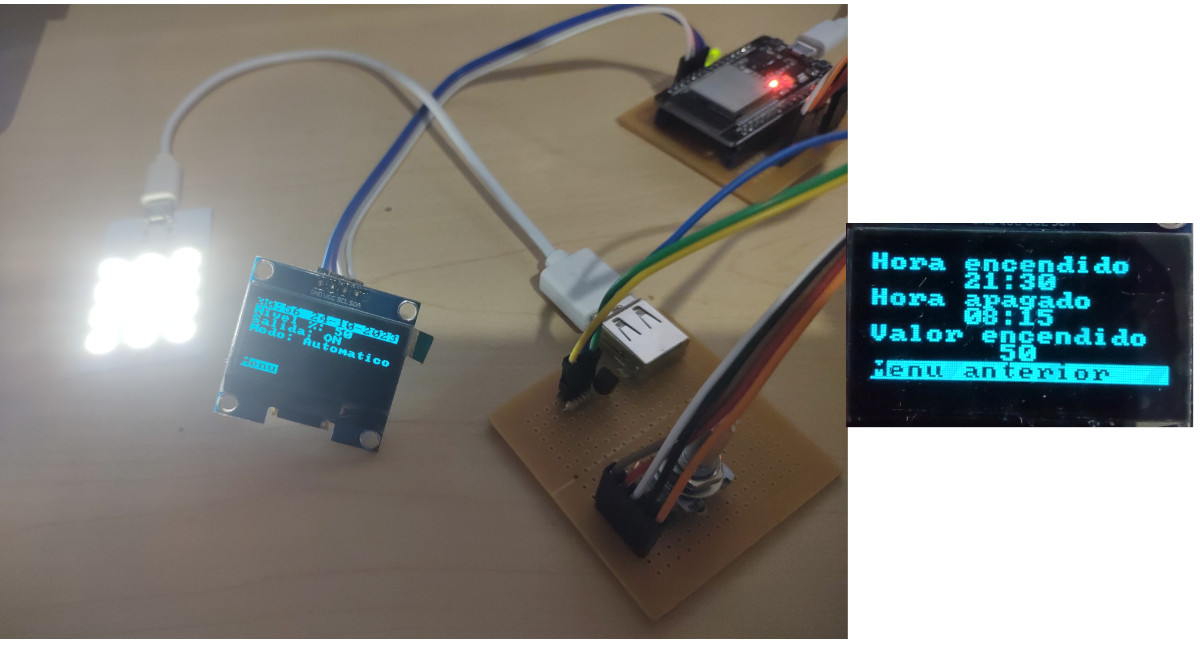
\includegraphics[scale=0.06]{Figura 37 - Dimmer funcionando.jpg}
\caption[Dimmer en modo automático funcionando]{Dimmer en modo automático funcionando.}
\label{fig:37}
\end{figure}

En la figura \ref{fig:38}, se puede observar la pantalla de configuración de modo automático.

\begin{figure}[h]
\centering
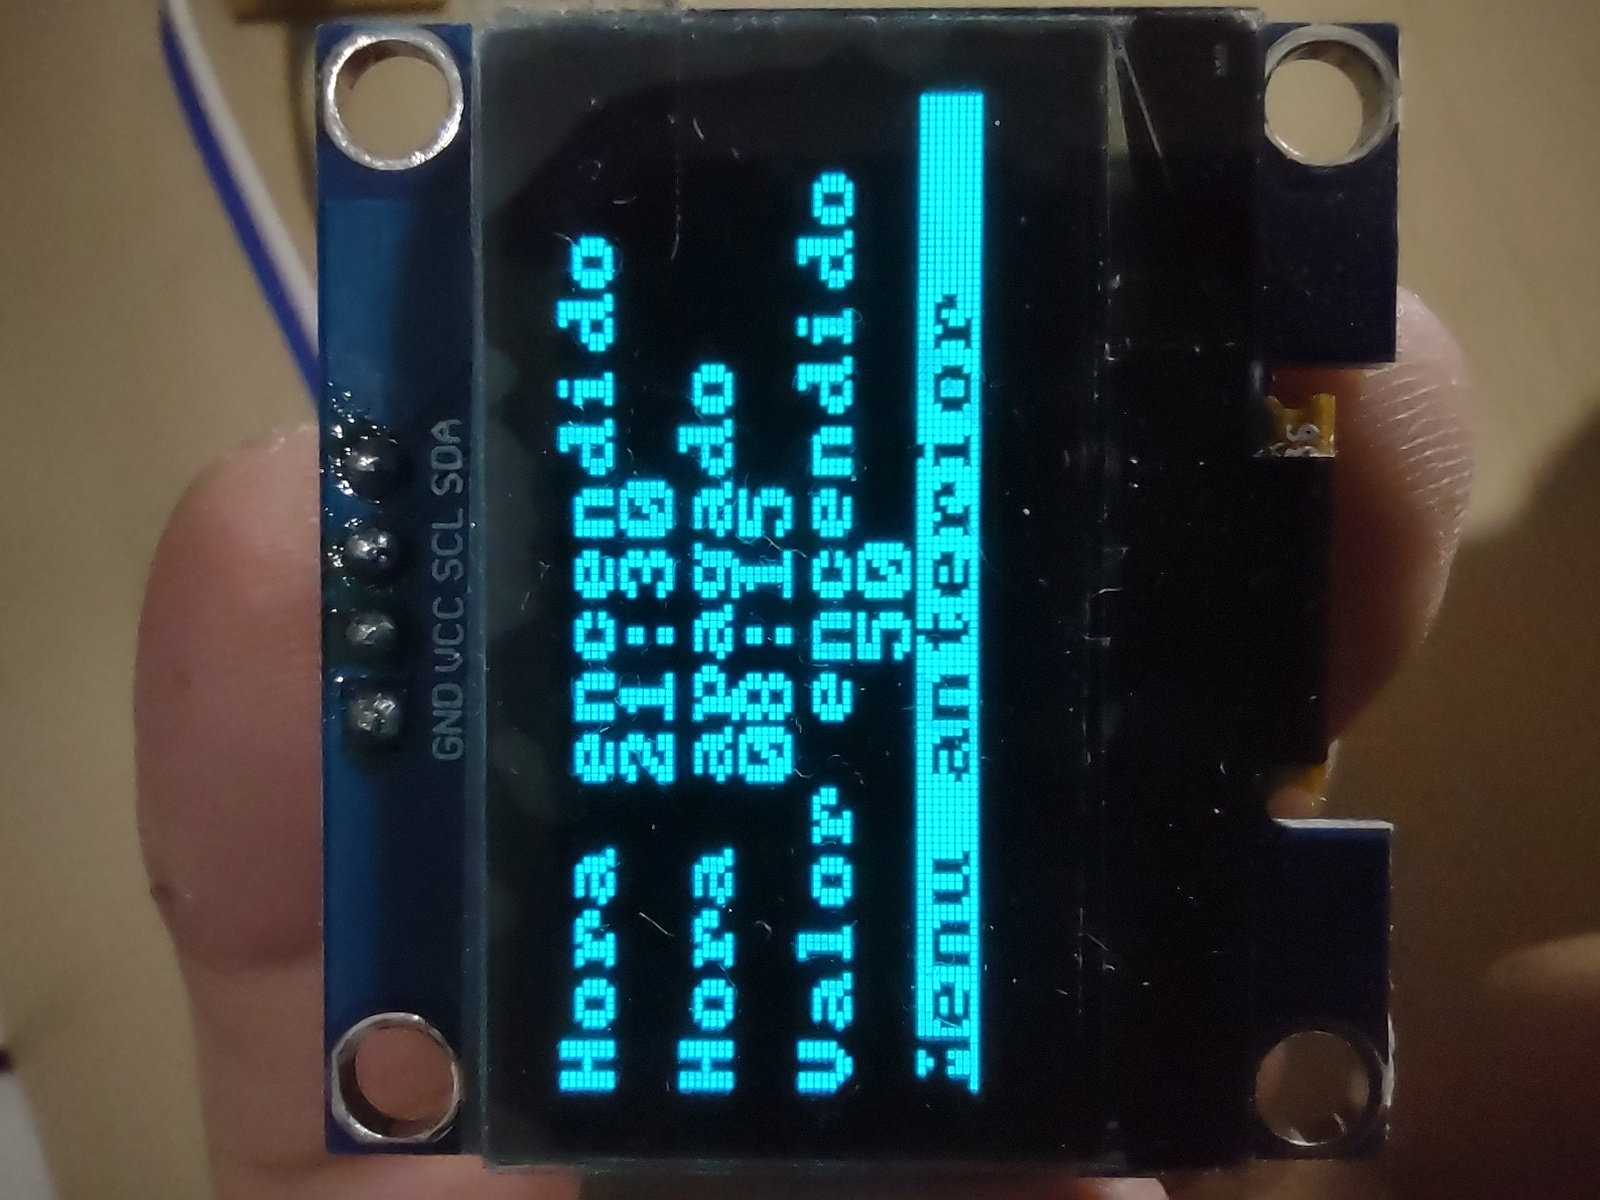
\includegraphics[angle=270, scale=0.47]{Figura 38 - Pantalla dimmer funcionando.jpg}
\caption[Pantalla de configuración del dimmer en modo automático]{Pantalla de configuración del dimmer en modo automático.}
\label{fig:38}
\end{figure}

En la figura \ref{fig:39} puede observarse la página de configuración del nodo dimmer. Puede observarse que los datos ingresados corresponden con los datos guardados en el nodo, y que este último está funcionando según lo esperado.

\begin{figure}[h]
\centering
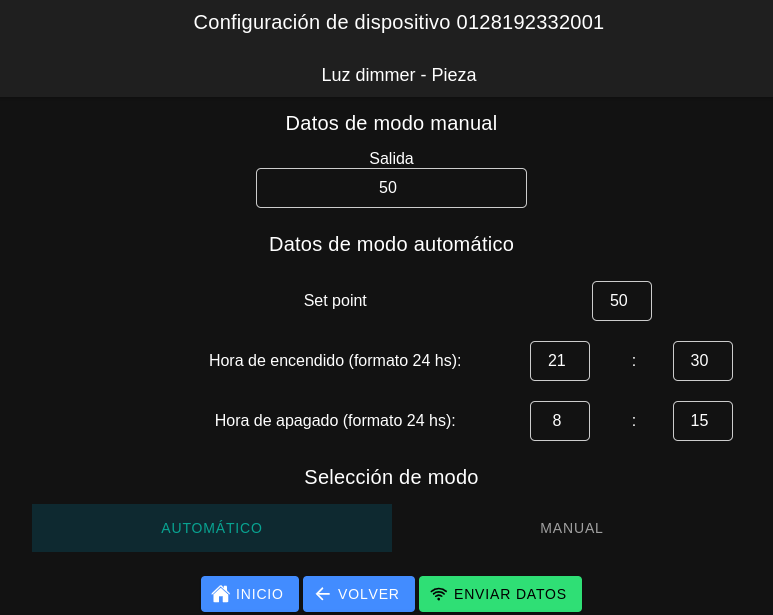
\includegraphics[scale=0.45]{Figura 39 - Config.png}
\caption[Pantalla de configuración de dimmer]{Pantalla de configuración de dimmer.}
\label{fig:39}
\end{figure}

Se ha verificado la capacidad de agregar y modificar los datos de los dispositivos desde la página correspondiente, contrastando los datos visualizados en la pantalla de \textit{phpMyAdmin}. Durante una prueba que se realizó, se cargó un dispositivo nuevo y se corroboró tanto desde la aplicación del sistema como desde la página de administración de la base de datos. En la figura \ref{fig:40} puede verse cómo se agregó un dispositivo nuevo desde la página en la parte superior y cómo se ve reflejado en la base de datos en la inferior.

\newpage
\begin{figure}[h]
\centering
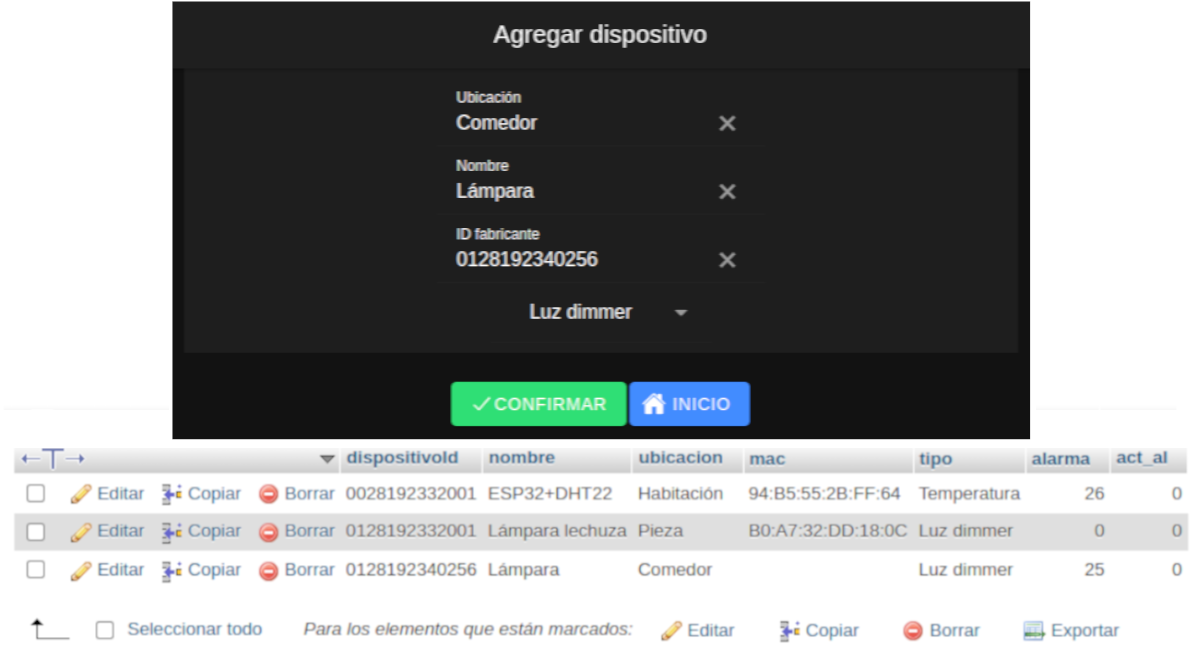
\includegraphics[scale=0.33]{Figura 40 - Agregar dispositivo.png}
\caption[Valores de dispositivo nuevo al agregar dispositivo]{Valores de dispositivo nuevo.}
\label{fig:40}
\end{figure}

Aquí se observa que los datos cargados coinciden con los almacenados. La diferencia radica en que no se registró la MAC del dispositivo ya que al momento de obtener la imagen el dispositivo no había emitido datos al servidor.

Algo similar a la prueba de los dispositivos se hizo con los usuarios. El sistema por default tiene los valores \textit{user1}, \textit{user2} y \textit{user3} y contraseña \textit{user}. Esto se logró creando estos usuarios con sus datos en el archivo de creación de la base de datos \textit{domotica.sql}. En la figura \ref{fig:41} se muestran los valores ingresados en la página de configuración en la parte superior y los que están almacenados en la base de datos en la inferior. Como se puede observar en la imagen, los valores cargados desde la página coinciden con los almacenados en la base de datos.

\begin{figure}[h]
\centering
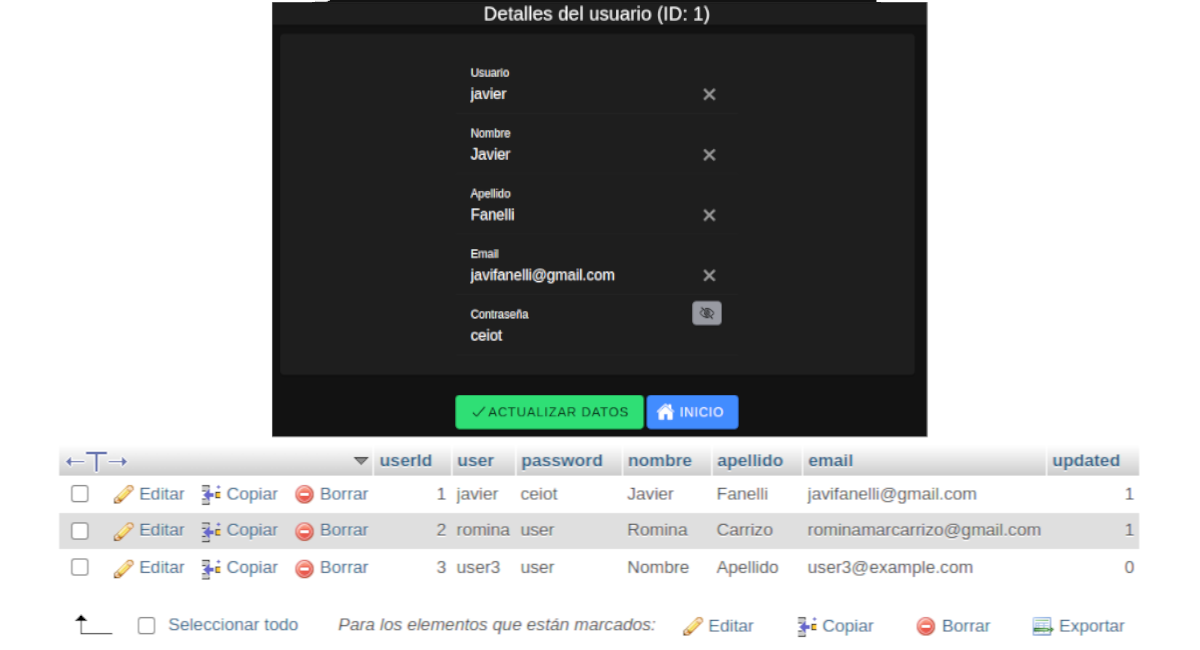
\includegraphics[scale=0.34]{Figura 41 - Modificar usuario.png}
\caption[Valores de usuario modificados]{Valores de usuario modificados.}
\label{fig:41}
\end{figure}

Por último, se hizo la corroboración de la activación de la alarma y el envío del mail. En la figura \ref{fig:42} puede observarse la configuración del dispositivo en la parte superior y el mail recibido en la parte inferior.

\begin{figure}[h]
\centering
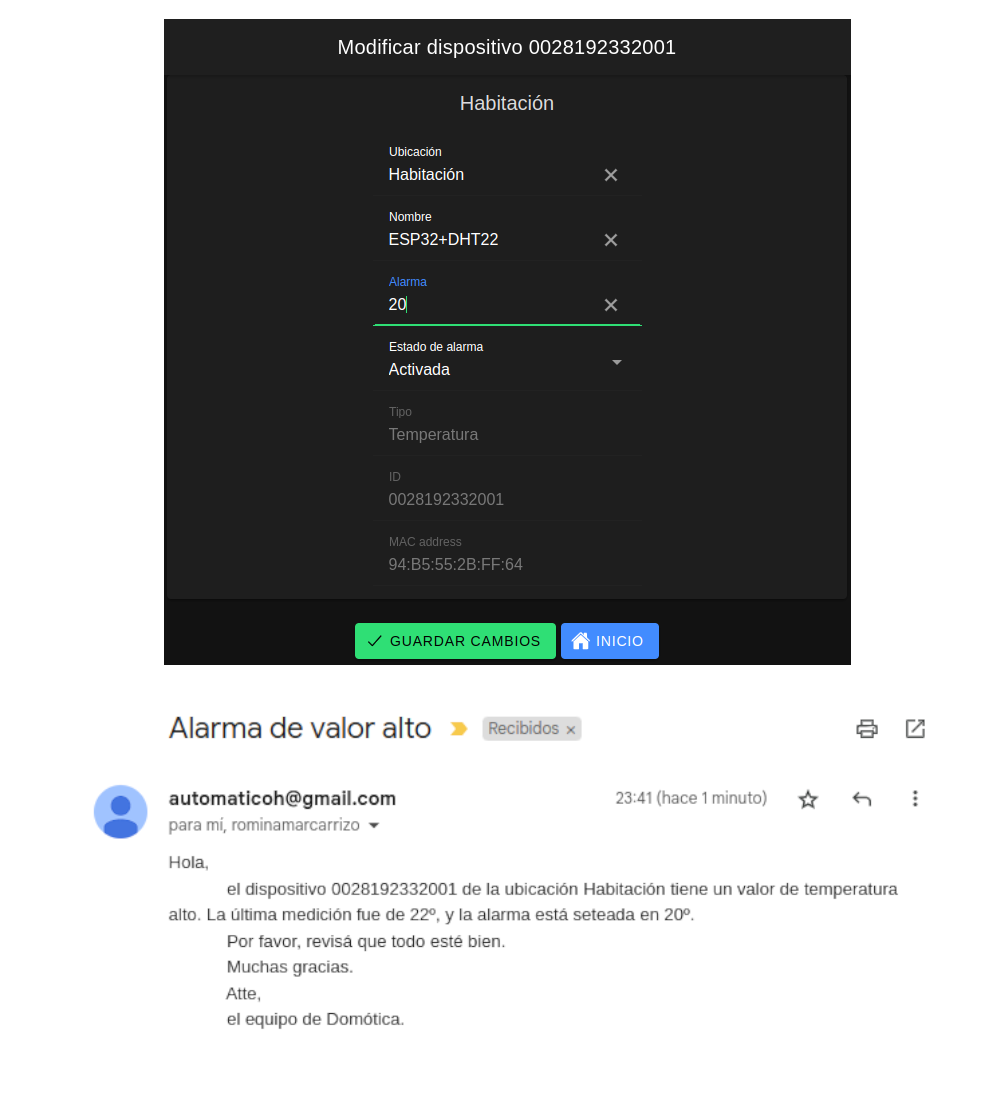
\includegraphics[scale=0.35]{Figura 42 - Alarma.png}
\caption[Envío de alarma de medición]{Envío de alarma de medición.}
\label{fig:42}
\end{figure}

De este modo, se realizaron las pruebas más importantes de funcionalidades del sistema. Al dar resultados de funcionamiento satisfactorios, se concluye que la aplicación funciona de manera correcta.

\section{Comparación con el estado del arte}

En la tabla \ref{tab:estadoarte} se encuentra la comparación entre las soluciones de hogares inteligentes existentes en el mercado nacional, Domotic y Reactor, y el trabajo realizado. 

\newpage
\begin{table}[h]
\centering
\caption[Comparativa entre las distintas opciones - Estado del arte]{Comparativa entre las distintas opciones.}
\begin{tabular}{l c c c}
\toprule
\textbf{Funcionalidad} & \textbf{Domotic} & \textbf{Reactor} & \textbf{Trabajo final}\\
\midrule
Posee unidad central			& Sí		& No		& Sí\\
Capacidad de diseño de		&		&		&\\
dispositivos nuevos			& Sí		& Sí		& Sí\\
Almacenamiento de mediciones	& No		& Sí		& Sí\\
Programación de reacciones	& Sí		& Sí		& Sí\\
Aplicación en ambientes		&		&		&\\
profesionales y oficinas		& No		& Sí		& Sí\\
Avisos por mail				& No		& Sí		& Sí\\
Aplicación móvil				& Sí		& Sí		& No\\
Conexión	 desde el exterior	& Sí		& Sí		& No\\
\bottomrule
\hline
\end{tabular}
\label{tab:estadoarte}
\end{table}

Como se puede observar de la tabla comparativa, el trabajo está a la par de otras soluciones similares. Entre sus puntos positivos, el sistema desarrollado posee una unidad central, en este caso, el servidor, que puede aceptar diseños nuevos de dispositivos, proporciona notificaciones en caso de eventos y almacena valores de mediciones que sean útiles.

En cuanto a los aspectos a mejorar se describirán en el capítulo 5 en la sección de trabajo futuro.